\documentclass[aspectratio=32]{beamer}
\usepackage[utf8]{inputenc}
\usepackage[ngerman]{babel}
\usepackage{amsmath}
\usepackage{amssymb}
\usepackage{amsthm}
\usepackage{mathtools}
\usepackage[T1]{fontenc}
\usepackage{graphicx}
\usepackage{lmodern}
\usepackage{stmaryrd} %Widerspruchspfeil
\usepackage{color}
\usepackage{xcolor}
%\usepackage{thmbox}
\usepackage{verbatim}
\usepackage{enumerate}
\usepackage{xifthen}
\usepackage{calc}
\usepackage{hyperref}
\usepackage[version=3,arrows=pgf-filled]{mhchem}
\usepackage[ruled, linesnumbered]{algorithm2e}
\usepackage{calrsfs}
\usepackage{bm}
\usepackage{float}

\title{Reaktions-Diffusions-Advektionsgleichung in 2D}
\author{Etienne Ott, Moritz Schleicher, Patrick Buchfink }
\institute{Numerische Simulation WS16/17}
\date{10. Februar 2017}


%Pakete für Quellcode importieren
\usepackage{listings}
\usepackage{listingsutf8}
%Einstellungen für Quellcode aus Matlab
\lstset{language=Matlab, breaklines=true, inputencoding=utf8/latin1}

%Umgebungen für Definition, Satz und Lemma
%\newtheorem[M]{defi}{Definition}
%\newtheorem[M]{satz}{Satz}
%\newtheorem[M]{lem}{Lemma}
\newtheorem{defi}{Definition}
\newtheorem{satz}[defi]{Satz}
\newtheorem{lem}[defi]{Lemma}
\newtheorem{kor}[defi]{Korollar}
\newtheorem{sud}[defi]{Satz und Definition}
\newtheorem{prop}[defi]{Proposition}
\newtheorem{bem}[defi]{Bemerkung}
\newtheorem{bsp}[defi]{Beispiel}

% Aufzaehlungszeichen
\newcommand{\blob}{\rule[2.2pt]{3pt}{3pt}}

%useful shortcuts
\newcommand{\N}{\ensuremath{\mathbb{N}}}
\newcommand{\Z}{\ensuremath{\mathbb{Z}}}
\newcommand{\Q}{\ensuremath{\mathbb{Q}}}
\newcommand{\R}{\ensuremath{\mathbb{R}}}
\newcommand{\C}{\ensuremath{\mathbb{C}}}
\newcommand{\E}{\ensuremath{\mathbb{E}}}
\newcommand{\Yt}{\ensuremath{\widetilde{Y}}}
\newcommand{\ft}{\ensuremath{\widetilde{f}}}
\newcommand{\bs}{\ensuremath{b^{\ast}}}
\newcommand{\Dn}[1]{\ensuremath{\widetilde{D}_{n,#1}}}
\newcommand{\cst}{\ensuremath{\text{cost}}}
\newcommand{\norm}[2][]{\ensuremath{\left\|#2\right\|_{#1}}} %allgemeine Norm
\newcommand{\inftynorm}[1]{\ensuremath{\norm[\infty]{#1}}}
\newcommand{\tnorm}[1]{\ensuremath{\norm[2]{#1}}}
\newcommand{\snorm}[2][]{\ensuremath{\left|#2\right|_{#1}}}
\newcommand{\scalarprod}[2]{\ensuremath{\left\langle{#1,#2}\right\rangle}} %Skalarprodukt
\newcommand{\farbig}[2][red]{\textcolor{#1}{#2}}
\newcommand{\sobolevnorm}[1]{\norm[W^{k,p}]{#1}}
\newcommand{\kpert}{\ensuremath{\kappa_\text{pert}}}
\newcommand{\trace}{\ensuremath{\operatorname{tr}}}
\renewcommand{\div}{\ensuremath{\operatorname{div}}}
\newcommand{\lpert}{\ensuremath{\lambda_\text{pert}}}
\newcommand{\mpert}{\ensuremath{\mu_\text{pert}}}

% standart calligrafic font
\DeclareMathAlphabet{\pazocal}{OMS}{zplm}{m}{n}
\newcommand{\calO}{\pazocal{O}}
\newcommand{\calH}{\pazocal{H}}
\newcommand{\calR}{\pazocal{R}}

%veränderter absatz
\parindent0em
\parskip=0.5\baselineskip


%Details for SimTech-Background
%\usepackage[loadonly]{enumitem}
%\setitemize{leftmargin=0.4cm}

\definecolor{simtechdarkblue}{HTML}{004884}
\definecolor{simtechbrightblue}{HTML}{BDC7DD}
\setbeamercolor{block title}{fg=white,bg = simtechdarkblue}
%\setbeamercolor{block body}{fg=black,bg=simtechdarkblue!10!white}
\setbeamercolor{block body}{fg=black,bg=simtechbrightblue!25!white}

\definecolor{simtechred}{HTML}{CF0000}

\usebackgroundtemplate{
\includegraphics[width=\paperwidth]{Vorlage_SimTech.pdf}}
\setbeamertemplate{frametitle}{
	\vspace*{1cm}
	\hspace*{0.1cm}
	\textcolor{simtechred}{\insertframetitle}
}

\setbeamertemplate{title page}{	
	\begin{center}
		\vspace*{2cm}
		\textcolor{simtechred}{{\LARGE\inserttitle}}\\[0.5cm]
		%\ifx\insertsubtitle\@empty\else\small\insertsubtitle \\[1cm]\fi
		\ifx\insertauthor\@empty\else\small\insertauthor \\\fi
		\ifx\insertinstitute\@empty\else\small\insertinstitute \\[0.3cm]\fi
		\small\insertdate
	\end{center}
}

\newcommand{\sectionframe}{\begin{frame}
	\begin{center}
		\textcolor{simtechred}{\Large\insertsection}
	\end{center}
\end{frame}}

% In case that parts are needed, use this
%\newcommand{\sectionframe}{\begin{frame}
%	\begin{center}
%		\textcolor{simtechred}{\LARGE Teil \insertsectionnumber \\\vspace{1cm}}
%		\textcolor{simtechred}{\LARGE\insertsection}
%	\end{center}
%\end{frame}}

\newcommand{\reditem}{\item[\textcolor{simtechred}{$\blob$}]}

%change color of enumerate items
\setbeamercolor{enumerate item}{fg = simtechdarkblue}

\setbeamertemplate{block begin}{%
  	\par\vskip\medskipamount
  	\leftskip=0.25cm%
  	\addtolength{\textwidth}{-\leftskip}
  	\begin{beamercolorbox}[colsep*=.75ex,wd=\textwidth]{block title}
    	\usebeamerfont*{block title}\insertblocktitle%
  	\end{beamercolorbox}%
  	{\parskip0pt\par}%
  	\ifbeamercolorempty[bg]{block title}
  	{}
  	{\ifbeamercolorempty[bg]{block body}{}{\nointerlineskip\vskip-0.5pt}}%
  	\leftskip=0.25cm
  	\usebeamerfont{block body}%
  	\begin{beamercolorbox}[colsep*=.75ex,vmode,wd=\textwidth]{block body}%
    \ifbeamercolorempty[bg]{block body}{\vskip-.25ex}{\vskip-.75ex}\vbox{}%
}

\setbeamertemplate{block end}{
\end{beamercolorbox}
}


\setbeamertemplate{theorems}[ams style]
\makeatletter\setbeamertemplate{theorem begin}{
\begin{block}{\textbf{\inserttheoremname \inserttheoremnumber}
\ifx\inserttheoremaddition\@empty\else[\inserttheoremaddition]\fi}
}\makeatother
\setbeamertemplate{theorem end}{\end{block}\par}
\setlength{\leftskip}{0.25cm}

% In case that parts are needed, use this
%\setbeamertemplate{section in toc}{
%\leavevmode\leftskip=0cm
%\textcolor{black}{\inserttocsection}\par
%}
\setbeamertemplate{section in toc}{
\leavevmode\leftskip=0cm
\textcolor{simtechred}{$\blob$}
\textcolor{black}{\inserttocsection}\par
}
\setbeamertemplate{subsection in toc}{
\leavevmode\leftskip=1cm
{\footnotesize\inserttocsubsection}\par
}

\beamertemplatenavigationsymbolsempty

%Framenumbering
% Diese sind optional, also kann die Zeile einfach auskommentiert werden
% um die Foliennummern abzustellen
\setbeamertemplate{footline}{\hfill\footnotesize\insertframenumber\hspace*{0.3cm}\vspace*{0.3cm}}


\begin{document}

\begin{frame}[plain]
\titlepage
\end{frame}

%framenumber neu setzen, damit nummerierung bei 1 anfängt.
\setcounter{framenumber}{0}

\begin{frame}
\frametitle{Inhalt}
\tableofcontents
\end{frame}

%----------------------------------------------------------------------------------
% Part 1: Einführung und Motivation
%----------------------------------------------------------------------------------
\section{Einführung und Motivation}
\sectionframe

\begin{frame}
\frametitle{Wiederholung: Diffusions-Advektionsgleichung}

\begin{center}
\begin{tabular}{ c c }
	Diffusion & Advektion \\
	\(
		\frac{\partial s(t,\bm{x})}{\partial t} = \nabla \cdot \left( \bm{D} \nabla s(t,\bm{x}) \right)
	\)
	&
	\(
		\frac{\partial s(t,\bm{x})}{\partial t} = - \nabla \cdot (\bm{v}s)
	\)
	\\
  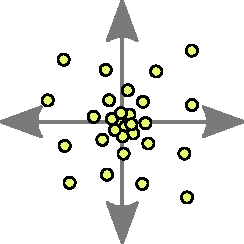
\includegraphics[width=\textwidth/3,keepaspectratio]{Bilder/diffusion.pdf}
	&
  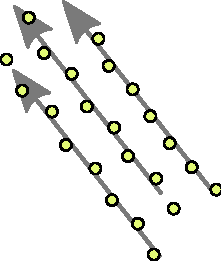
\includegraphics[width=\textwidth/3,keepaspectratio,angle=-90,origin=c]{Bilder/advection.pdf}
	\\
\end{tabular}
\end{center}

\end{frame}

\begin{frame}
\frametitle{Motivation: Reaktionen}

\begin{center}
\begin{tabular}{ c }
	Reaktion \\
	\(
		\frac{\partial s(t,\bm{x})}{\partial t} = R(s,t,\bm{x})
	\)
	\\
	
\includegraphics[height=\textwidth/4,keepaspectratio,angle=-90]{Bilder/population.pdf}
	\\
  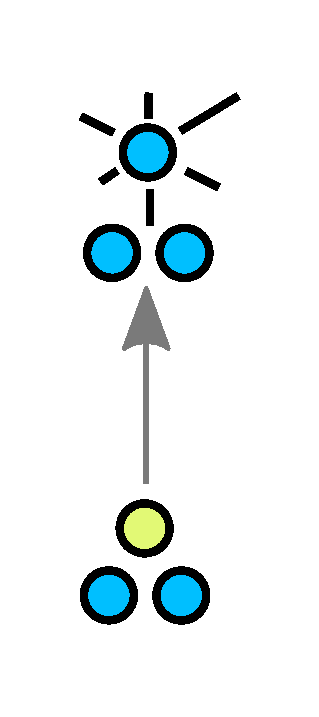
\includegraphics[height=\textwidth/4,angle=-90]{Bilder/reaction.pdf}
	\\
\end{tabular}
\end{center}

\end{frame}

%----------------------------------------------------------------------------------
% Part 2: Theorie: Populationsdynamik 
%----------------------------------------------------------------------------------
\section{Theorie: Populationsdynamik}
\sectionframe

\begin{frame}
\frametitle{Idee der Populationsdynamik}

\begin{tabular}{c}
	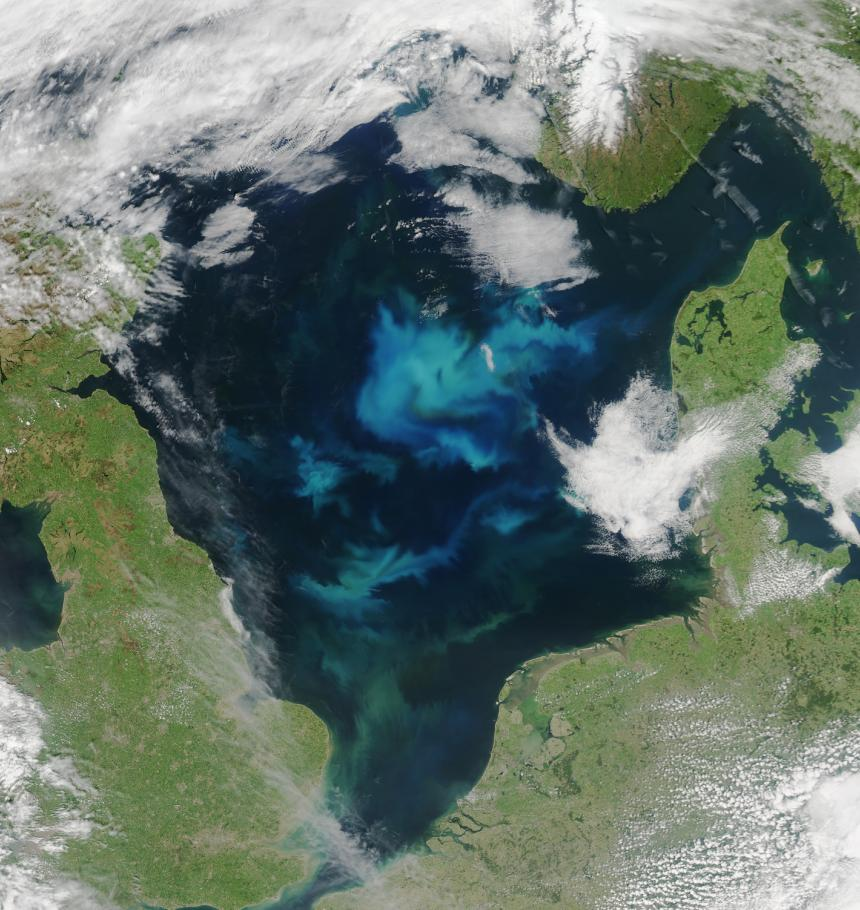
\includegraphics[height=\textheight/3*2,keepaspectratio]{Bilder/seaweed.jpg}
	\\
	{\small \textit{Quelle: http://www.spiegel.de/wissenschaft/natur/bild-1042982-869697.html}}
	\\
\end{tabular}

\end{frame}

%----------------------------------------------------------------------------------
% Part 3: Theorie: Gray-Scott Modell 
%----------------------------------------------------------------------------------
\section{Theorie: Gray-Scott Modell}
\sectionframe

\begin{frame}
\frametitle{Idee des Gray-Scott Modells}
\begin{itemize}
  \reditem Zwei Substanzen A: Futter, B: Räuber
%    \begin{figure}[!H]
%      
\includegraphics[height=\textwidth/12,keepaspectratio,angle=-90,origin=c]{Bilder/substances.pdf}
%    \end{figure}
  \reditem Phänomene
\begin{tabular}{ r c c c }
	& Feed & Reaktion & Kill \\
	&
  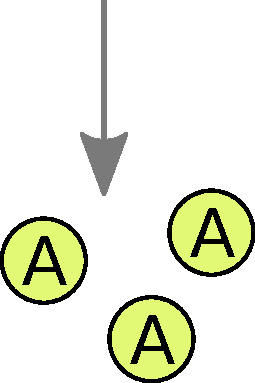
\includegraphics[height=\textwidth/6,keepaspectratio]{Bilder/gs_feed.pdf}
	&
  
\includegraphics[height=\textwidth/6,keepaspectratio,angle=-90,origin=c]{Bilder/gs_reaction.pdf}
  &
  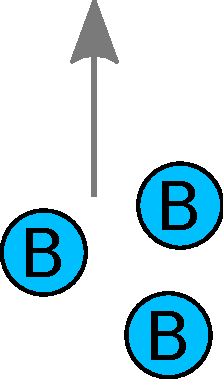
\includegraphics[height=\textwidth/6,keepaspectratio]{Bilder/gs_kill.pdf}
	\\
	\(
		R_A(s_A,s_B,t,\bm{x})=
	\)
	&
	\(
		f(1-s_A)
	\)
	&
	\(
		- s_A s_B^2
	\)
	&
	\\
	\(
		R_B(s_A,s_B,t,\bm{x})=
	\)
	&
	&
	\(
		+ s_A s_B^2
	\)
	&
	\(
		- (k + f) s_B
	\)
	\\
\end{tabular}

  \reditem Parameter
\begin{itemize}
	\item Kill-Rate $k$
	\item Feed-Rate $f$
	\item Diffusions-Konstanten $d_A, d_B$
\end{itemize}
    
\end{itemize}
\end{frame}

\begin{frame}
\frametitle{Gray-Scott Modell ohne Advektion}

\begin{itemize}
	\reditem Muster bekannt von
\begin{itemize}
	\item	Blättern
	\item Tierfellen (Rehe, Giraffen, Schmetterlinge, ...)
	\item Miktose
\end{itemize}
\end{itemize}
\begin{tabular}{l}
	
\includegraphics[width=\textwidth,keepaspectratio]{Bilder/gs_scenarios.png} \\
	\textit{Quelle: http://www.karlsims.com/rd.html} \\
\end{tabular}

\end{frame}

%----------------------------------------------------------------------------------
% Part 3: Implementierung 
%----------------------------------------------------------------------------------
\section{Implementierung}
\sectionframe

\begin{frame}
\frametitle{Implementierung der Substanzen und deren Reaktionsterms}
% Variables Einlesen der Anfangsbedingung
% Wie werden Substanzen gespeichert?
% Wann wird Reaktionsterm berechnet?
% 	d.h.: an welcher Stelle in der Simulationspiple?
% Wie werden Randbedingungen gewählt?

\end{frame}

%----------------------------------------------------------------------------------
% Part 4: Ergebnisse 
%----------------------------------------------------------------------------------
\section{Ergebnisse}
\sectionframe

\begin{frame}
\frametitle{Ergebnisse - Populationsdynamik}

\end{frame}

\begin{frame}
\frametitle{Ergebnisse - Gray-Scott Modell}
% Videos von Hand abspielen

\end{frame}

%%----------------------------------------------------------------------------------
%% Part 5: Zusammenfassung 
%%----------------------------------------------------------------------------------
%\section{Zusammenfassung}
%\sectionframe
%
%\begin{frame}
%\frametitle{Zusammenfassung: Reaktions-Diffusions-Advektionsgleichung in 2D}
%
%\end{frame}

%% Black Frame
%\addtocounter{framenumber}{-1} %correct framenumber
%\bgroup
%\setbeamertemplate{background canvas}[default]
%\setbeamercolor{background canvas}{bg=black}
%\begin{frame}[plain]{}
%\end{frame}
%\egroup

%Closing Frame
\begin{frame}
\begin{center}
\Large
\textcolor{simtechred}{Danke für die Aufmerksamkeit! \\ Fragen?}
\end{center}
\end{frame}
\end{document}
